
\section{Introduzione} % Sections are added in order to organize your presentation into discrete blocks, all sections and subsections are automatically output to the table of contents as an overview of the talk but NOT output in the presentation as separate slides

%------------------------------------------------

\begin{frame}
\frametitle{Le funzioni di hash}

Una funzione di hash prende in input un messaggio di lunghezza arbitraria e restituisce un valore di lunghezza prefissata chiamata hash o digest.

Queste funzioni sono utilizzate negli ambiti in cui ci sia la necessità di verificare l'integrità dei dati.
\vspace{1cm}
\begin{center}
    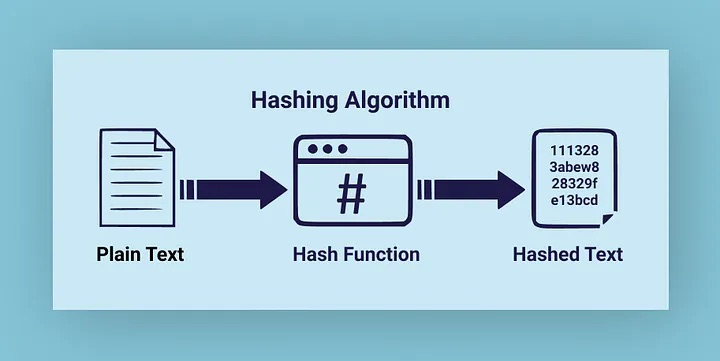
\includegraphics[width=0.5\textwidth]{img/1-img/hash-function.jpeg}
\end{center}
    

\end{frame}

\begin{frame}
\frametitle{Fefinizione funzione di hash}

Dato un alfabeto $\mathfrak{A}$, indicheremo con $\mathfrak{A}^*$ l’insieme di tutte le stringhe finite di elementi di $\mathfrak{A}$

\[
\emptyset^* = \bigcup_{n \geq 1} \mathfrak{A}^n
\]

Tipicamente $\mathfrak{A} = \{0, 1\}$, e quindi $\mathfrak{A}^*$ è l’insieme di tutte le stringhe composte da bit.

\vspace{1cm}
Una funzione hash è una funzione $h : \mathfrak{A}^* \rightarrow \mathfrak{B}^n$ che mappa stringhe di lunghezza arbitraria in stringhe di lunghezza fissa $n$ (per esempio n = 160)

\end{frame}


\begin{frame}
\frametitle{Proprietà delle funzioni di hash}

\begin{itemize}
    \item \textbf{Determinismo}: per uno stesso input la funzione restituisce sempre lo stesso output.
    \item \textbf{Velocità}: la funzione deve essere veloce da calcolare.
    \item \textbf{Difficoltà di inversione}: data l'uscita della funzione è computazionalmente difficile trovare l'input.
    \item \textbf{Effetto valanga}: piccole variazioni nell'input devono produrre grandi variazioni nell'output.
    \item \textbf{Resistenza alle collisioni}: è computazionalmente difficile trovare due input diversi che producano lo stesso output.
\end{itemize}
\end{frame}

\begin{frame}
\frametitle{Preimage resistence}
\textbf{Prima (debole) resistenza alla preimmagine}:
\begin{itemize}
    \item per quasi tutti gli output pre-specificati, è computazionalmente infattibile trovare un qualsiasi input che venga hashato a quell'output.
    Avendo \( y \), è difficile trovare un \( x \) tale che \( h(x) = y \).
\end{itemize}
\textbf{Seconda (forte) resistenza alla preimmagine}:
\begin{itemize}
    \item per un input specificato, è computazionalmente infattibile trovare un altro input che produca lo stesso output.
     Avendo \( x \), è difficile trovare un secondo input \( x' \neq x \) tale che \( h(x) = h(x') \).
\end{itemize}

\end{frame}

\begin{frame}
\frametitle{Secure Hash Algorithm: SHA-1}

La specifica originale è stata pubblicata nel 1993 come \textbf{Secure Hash Standard} dal National Institute of Standards and Technology.
SHA-0 fu ritirato dall'NSA e sostituito da una versione rivista dopo 2 anni quando fu pubblicato SHA-1 che prevedeva una rotazione di bit in più
per correggere un difetto nell'algoritmo originale.

\vspace{1cm}

I digest prodotti da SHA-1 sono di \textbf{160 bit}, e ogni messaggio può essere al massimo di \textbf{\(2^{64} - 1\) bit}.
\end{frame}

\begin{frame}
\frametitle{Secure Hash Algorithm: Funzionamento}
\begin{itemize}
    \item \textbf{Padding}: il messaggio viene convertito in binario e viene aggiunto un bit 1 seguito da zeri fino a che la lunghezza del messaggio è congrua a 448 modulo 512.
    \item \textbf{Lunghezza}: viene aggiunta la lunghezza del messaggio originale in binario a 64 bit.
    Al termine del primi 2 passaggi si avrà un messaggio con una lunghezza multipla di 512 bit.
    \item \textbf{Registri}: vengono inizializzati 5 registri da 32 bit con dei valori fissi.
    \begin{itemize}
        \item A = 67452301
        \item B = EFCDAB89
        \item C = 98BADCFE
        \item D = 10325476
        \item E = C3D2E1F0
    \end{itemize}
\end{itemize}
\end{frame}

\begin{frame}
\frametitle{Secure Hash Algorithm: Funzionamento P2}
\begin{itemize}
    \item \textbf{Elaborazione dei blocchi}: 
    \begin{itemize}
        \item I blocchi di 512 bit vengono divisi in 16 parole da 32 bit.
        \item Funzione di compressione che è formata da 4 cicli di 20 passi cadauno.
        \item Alla fine di ogni blocco i registri vengono aggiornati con i valori ottenuti.
    \end{itemize}
\end{itemize}

\begin{center}
    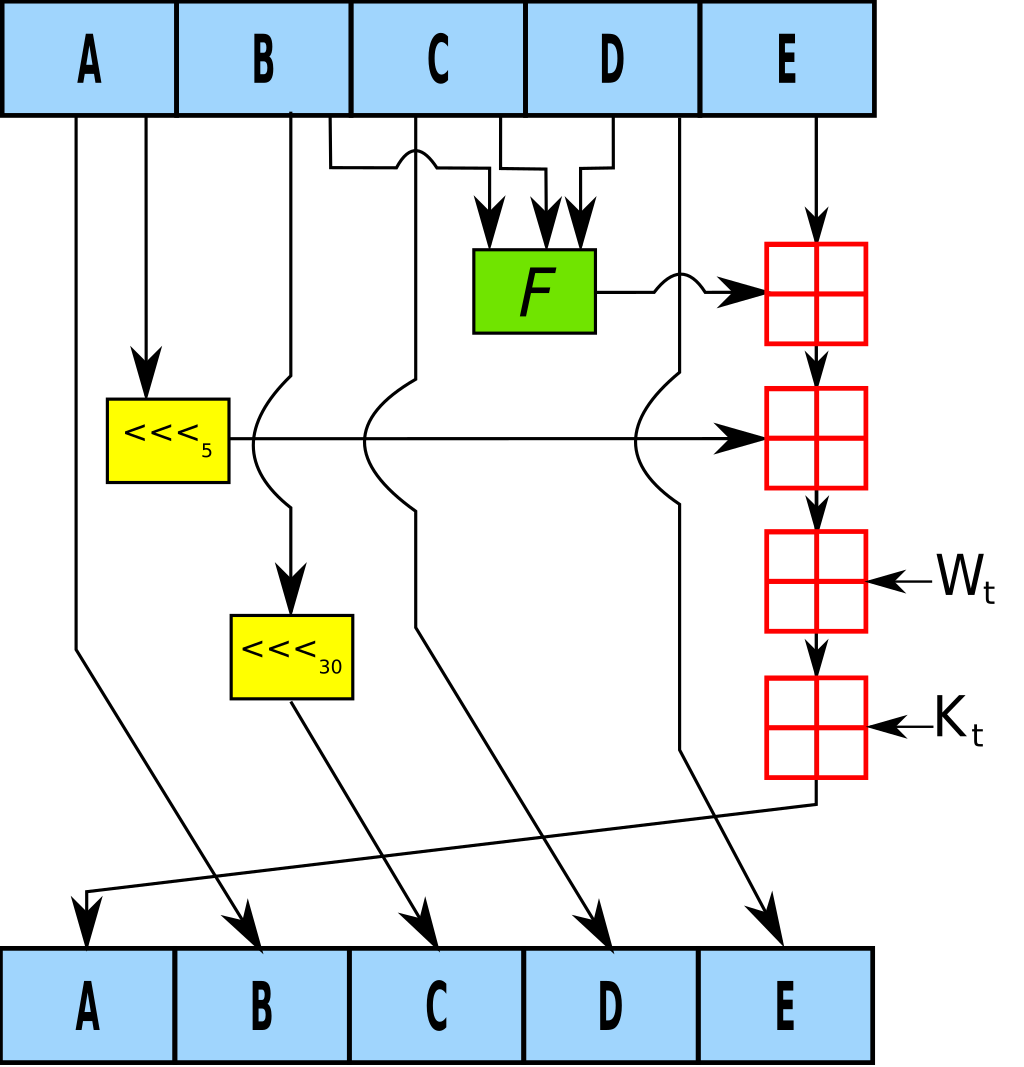
\includegraphics[width=0.4\textwidth]{img/1-img/SHA-1.png}
\end{center}

\end{frame}

\begin{frame}
    \frametitle{Firma digitale con PGP}
PGP calcola un hash dal testo in chiaro, e crea poi da questo hash la firma digitale usando la  \textbf{chiave privata del mittente}.
\begin{center}
    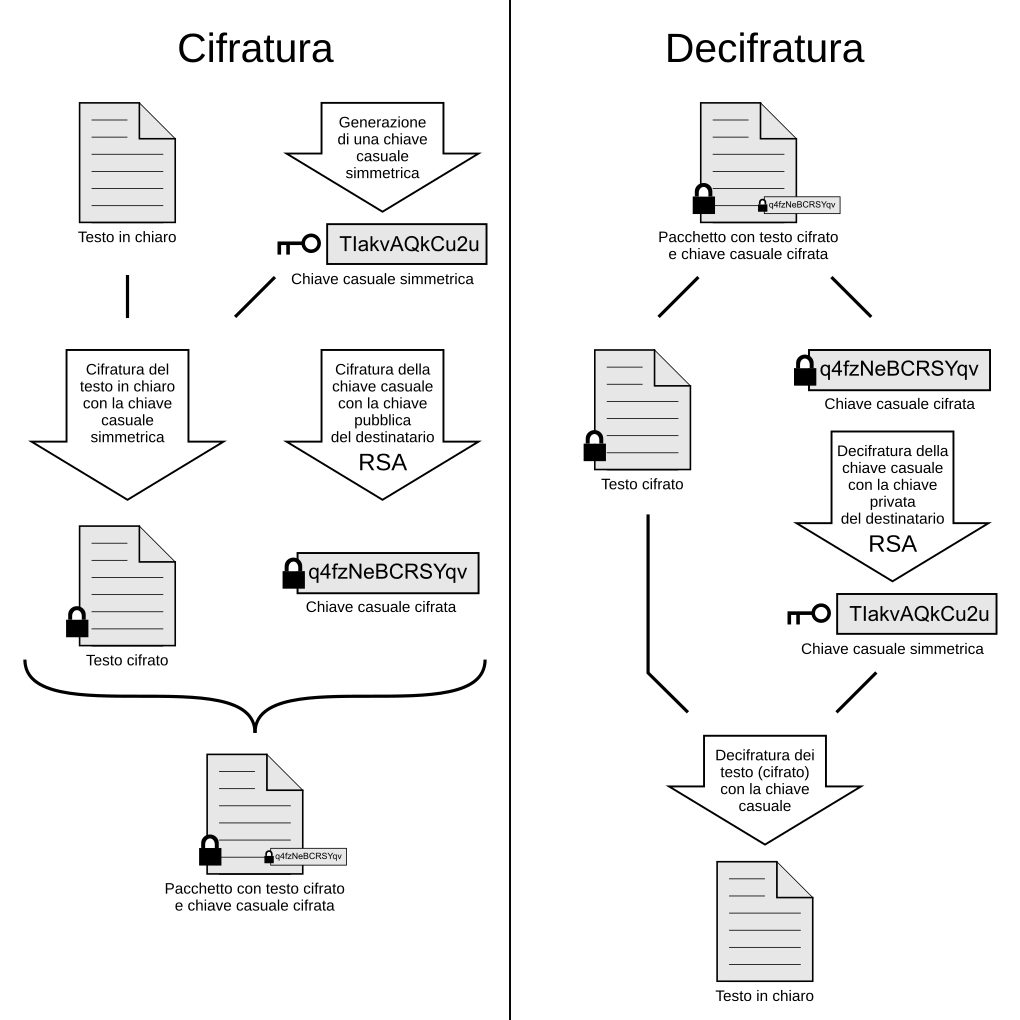
\includegraphics[width=0.5\textwidth]{img/1-img/PGP_diagram_IT.png}
\end{center}
\end{frame}

\begin{frame}
    \frametitle{Firma digitale con PGP Parte 2}
Il destinatario del messaggio calcola il message digest dal testo in chiaro decifrato, e poi usa la \textbf{chiave pubblica del mittente} ed il valore del message digest e la firma.
In questo modo si può verificare che il messaggio non sia stato alterato e che sia stato inviato dal mittente.

\begin{center}
    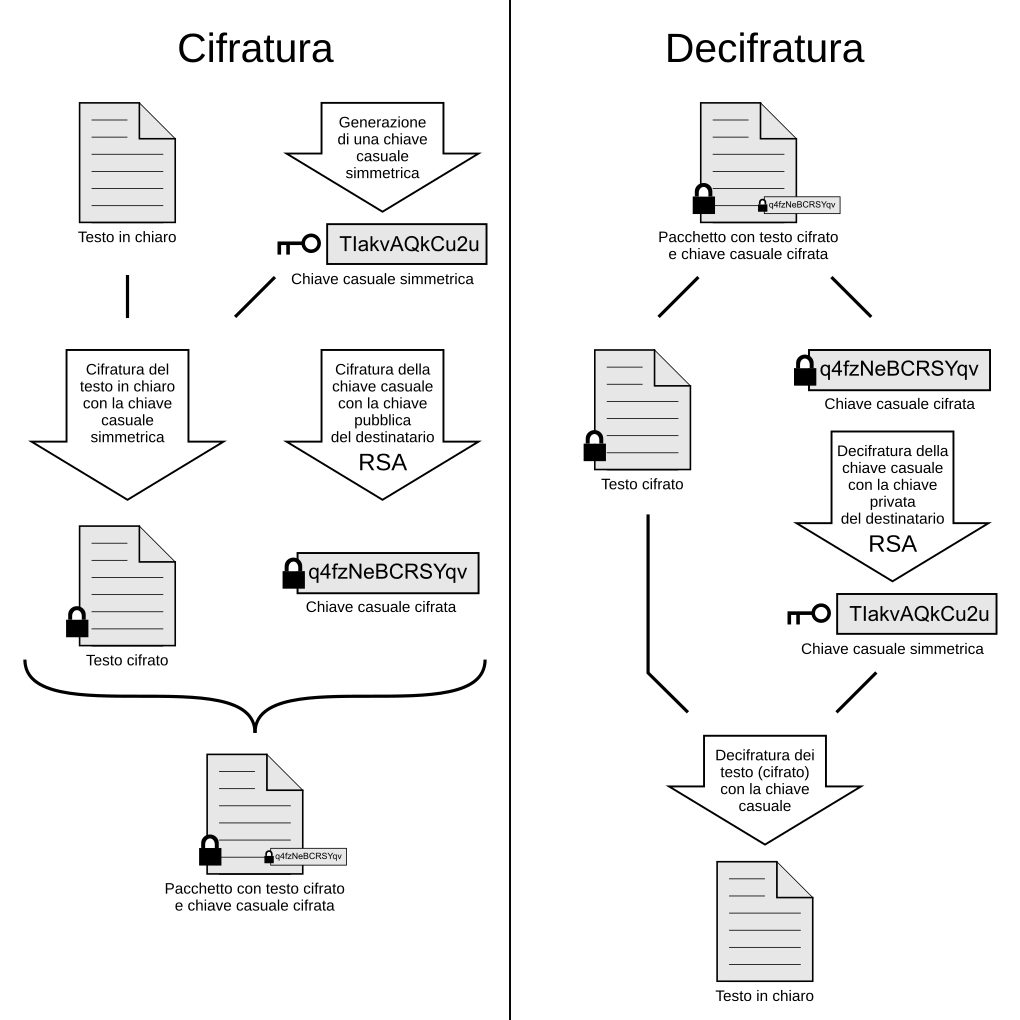
\includegraphics[width=0.5\textwidth]{img/1-img/PGP_diagram_IT.png}
\end{center}
\end{frame}